\documentclass[letterpaper,12pt,fleqn]{article}
\usepackage{matharticle}
\usepackage{pgfplots}
\usepackage{siunitx}
\pgfplotsset{compat=1.14}
\pagestyle{plain}
\begin{document}

\begin{center}
\Large Math-1003b Practice Exam \#1
\end{center}

\begin{enumerate}
  \newcommand{\ans}{\rule{0.5in}{1pt}}

\item Match the following nine functions with the correct graph show below. Find
  the graph that matches each function and write the letter for that graph
  to the right of the corresponding function.

  \vspace{0.25in}

  \begin{minipage}[t]{3in}
    \begin{tabular}{lc}
      $f(x)=x$ & \ans \\
      \\
      $f(x)=x^2$ & \ans \\
      \\
      $f(x)=x^3$ & \ans \\
      \\
      $f(x)=\sqrt{x}$ & \ans \\
      \\
      $f(x)=\frac{1}{x}$ & \ans \\
    \end{tabular}
  \end{minipage}
  \begin{minipage}[t]{3in}
    \begin{tabular}{lc}
      $f(x)=\abs{x}$ & \ans \\
      \\
      $f(x)=-1$ & \ans \\
      \\
      $f(x)=x-2$ & \ans \\
      \\
      $f(x)=-x^2+x+1$ & \ans \\
    \end{tabular}
  \end{minipage}

  \vspace{0.25in}

  \begin{tabular}{ccc}
    \begin{tikzpicture}
      \draw [<->] (-2,0) -- (2,0);
      \draw [<->] (0,-2) -- (0,2);
      \draw [domain=-1.25:1.25] plot (\x,{(\x)^3});
      \node at (-2,2) {$g)$};
    \end{tikzpicture} \hspace{0.25in} &
    \begin{tikzpicture}
      \draw [<->] (-2,0) -- (2,0);
      \draw [<->] (0,-2) -- (0,2);
      \draw [domain=-1.4:1.4] plot (\x,{(\x)^2});
      \node at (-2,2) {$f)$};
    \end{tikzpicture} \hspace{0.25in} &
    \begin{tikzpicture}
      \draw [<->] (-2,0) -- (2,0);
      \draw [<->] (0,-2) -- (0,2);
      \draw [domain=0:2] plot (\x,{sqrt(\x)});
      \node at (-2,2) {$a)$};
    \end{tikzpicture} \\
  \end{tabular}

  \begin{tabular}{ccc}
    \begin{tikzpicture}
      \draw [<->] (-2,0) -- (2,0);
      \draw [<->] (0,-2) -- (0,2);
      \draw [domain=-2:2] plot (\x,{(\x)});
      \node at (-2,2) {$d)$};
    \end{tikzpicture} \hspace{0.25in} &
    \begin{tikzpicture}
      \draw [<->] (-2,0) -- (2,0);
      \draw [<->] (0,-2) -- (0,2);
      \draw [domain=-2:2] plot (\x,{-1/2});
      \node at (-2,2) {$e)$};
    \end{tikzpicture} \hspace{0.25in} &
    \begin{tikzpicture}
      \draw [<->] (-2,0) -- (2,0);
      \draw [<->] (0,-2) -- (0,2);
      \draw [domain=-2:2] plot (\x,{abs(\x)});
      \node at (-1,2) {$i)$};
    \end{tikzpicture} \\
  \end{tabular}

  \begin{tabular}{ccc}
    \begin{tikzpicture}
      \draw [<->] (-2,0) -- (2,0);
      \draw [<->] (0,-2) -- (0,2);
      \draw [domain=-1:2] plot (\x,{-(\x)^2+(\x)+1});
      \node at (-2,2) {$h)$};
    \end{tikzpicture} \hspace{0.25in} &
    \begin{tikzpicture}
      \draw [<->] (-2,0) -- (2,0);
      \draw [<->] (0,-2) -- (0,2);
      \draw [domain=-1:2] plot (\x,{(\x)-1});
      \node at (-2,2) {$c)$};
    \end{tikzpicture} \hspace{0.25in} &
    \begin{tikzpicture}
      \draw [<->] (-2,0) -- (2,0);
      \draw [<->] (0,-2) -- (0,2);
      \draw [domain=0.5:1.9] plot (\x,{1/\x});
      \draw [domain=-1.9:-0.5] plot (\x,{1/\x});
      \node at (-2,2) {$b)$};
    \end{tikzpicture} \\
  \end{tabular}

  \newpage

\item Use the graph of $A(x)$ to answer the following questions:

  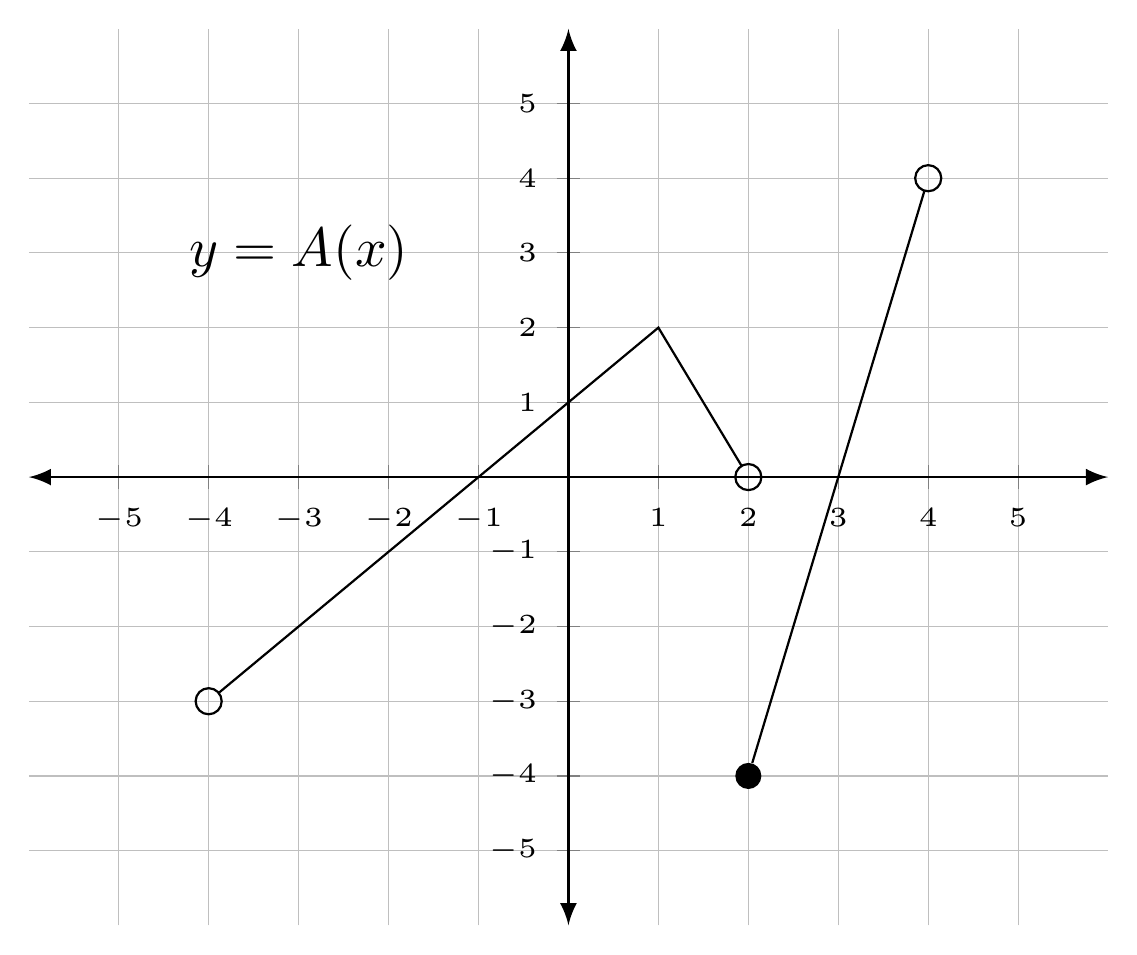
\begin{tikzpicture}[scale=2]
    \begin{axis}[
        xmin=-6,xmax=6,
        ymin=-6,ymax=6,
        grid=both,
        grid style={line width=.1pt, draw=gray!10},
        major grid style={line width=.2pt,draw=gray!50},
        axis lines=middle,
        axis line style={latex-latex},
        xtick={-5,-4,-3,-2,-1,0,1,2,3,4,5},
        ytick={-5,-4,-3,-2,-1,0,1,2,3,4,5},
        ticklabel style={font=\tiny},
      ]
      \node (a) [circle,draw,scale=0.5] at (-4,-3) {};
      \node (b) [circle,draw,scale=0.5] at (2,0) {};
      \node (c) [circle,fill,scale=0.5] at (2,-4) {};
      \node (d) [circle,draw,scale=0.5] at (4,4) {};
      \draw (a) to (1,2) to (b);
      \draw (c) to (d);
      \node at (-3,3) {$y=A(x)$};
    \end{axis}
  \end{tikzpicture}

  \begin{enumerate}
  \item What is $A(2)$?

    \vspace{0.5in}

  \item What is the y-intercept?

    \vspace{0.5in}

  \item For what values of $x$ is $A(x)=0$?

    \vspace{0.5in}

  \item What is the domain of $A$, in interval notation?

    \vspace{0.5in}

  \item What is the range of $A$, in interval notation?
  \end{enumerate}

  \newpage
  
\item Given the function: $f(x)=-2x+3$:
  \begin{enumerate}
  \item Is $f$ constant, linear, quadratic, or none of these?

    \vspace{0.5in}

  \item Find the y-intercept(s) of $f$.

    \vspace{1.0in}

  \item Find the x-intercepts(s) of $f$.

    \vspace{1.0in}

  \item Plot the intercepts of $f$ on the axes below and label the
    coordinates. Also draw the complete graph of $f$.
    
    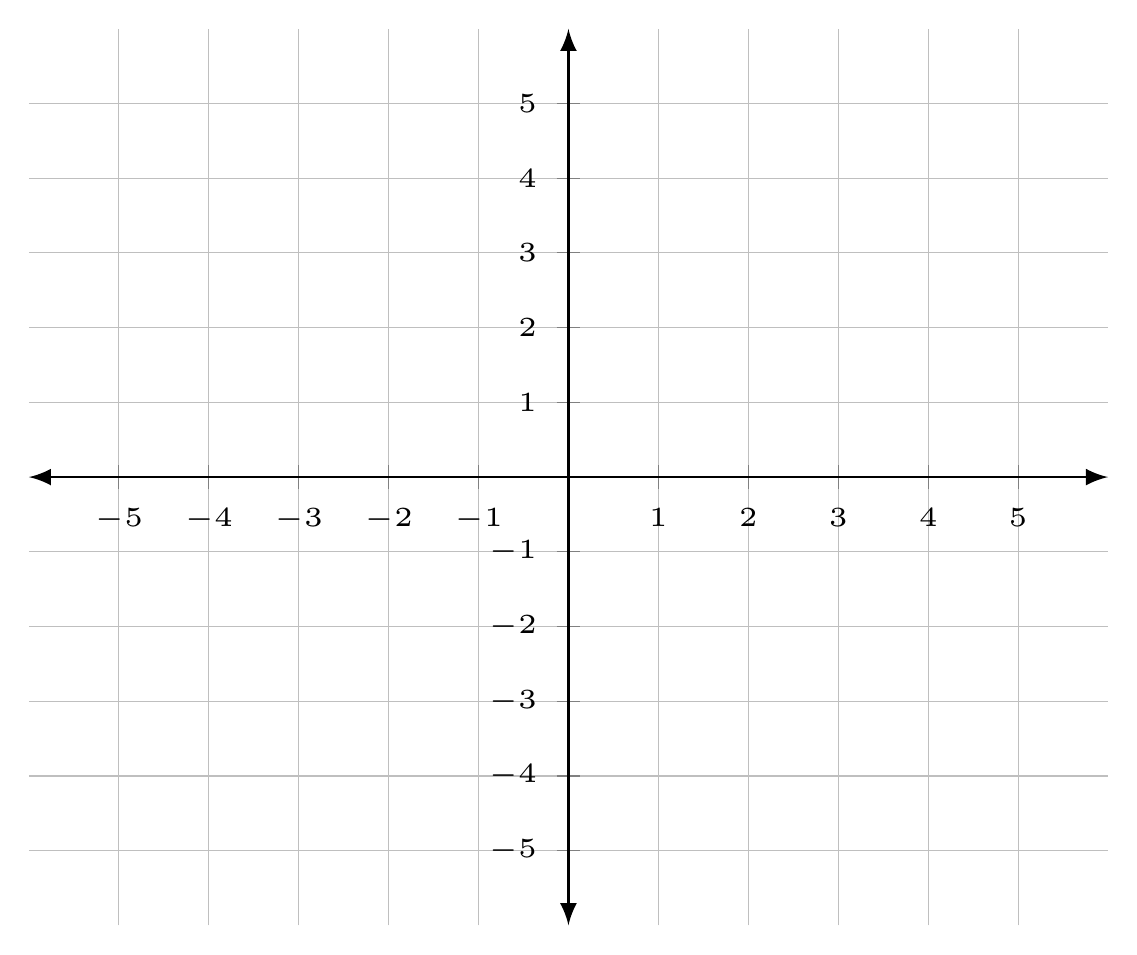
\begin{tikzpicture}[scale=2]
      \begin{axis}[
          xmin=-6,xmax=6,
          ymin=-6,ymax=6,
          grid=both,
          grid style={line width=.1pt, draw=gray!10},
          major grid style={line width=.2pt,draw=gray!50},
          axis lines=middle,
          axis line style={latex-latex},
          xtick={-5,-4,-3,-2,-1,0,1,2,3,4,5},
          ytick={-5,-4,-3,-2,-1,0,1,2,3,4,5},
          ticklabel style={font=\tiny},
        ]
    \end{axis}
  \end{tikzpicture}
  \end{enumerate}

  \newpage
  
\item The proposed California Bullet Train can make the $\SI{450}{mile}$ trip
  from Los Angeles to San Francisco in the same time that it takes a regular
  AMTRAK train to go just $\SI{135}{miles}$. How fast does each train go if the
  bullet train goes $\SI{140}{mph}$ faster than AMTRAK?

  \vspace{0.25in}

\item Perform the operation:
  \[\frac{2}{3-t}+\frac{t}{t^2-9}\]

\item Perform the operation:
  \[\frac{2x+6}{5x-15}\cdot\frac{4(x-3)}{x^2+6x+9}\]

\item Perform the operation:
  \[\frac{\frac{6-5y}{4y}}{5-\frac{6}{y}}\]

\item Solve for $w$:
  \[\frac{w}{12}+\frac{w+3}{3w}=\frac{1}{w}\]

  \vspace{0.25in}

\item Given:
  \begin{eqnarray*}
    f(x) &=& x-5 \\
    g(x) &=& x^2-5x
  \end{eqnarray*}
  Do the following:
  \begin{enumerate}
  \item What is $(f+g)(x)$ and its domain?
  \item What is $(f-g)(x)$ and its domain?
  \item What is $(fg)(x)$ and its domain?
  \item What is $\left(\frac{f}{g}\right)(x)$ and its domain?
  \item What is $(f\circ g)(x)$ and its domain?
  \item What is $(g\circ f)(x)$ and its domain?
  \item What is $(f\circ g)(1)$?
  \end{enumerate}

\end{enumerate}

\end{document}
